\documentclass[10pt,a4paper]{book}
\usepackage{amsmath}
\usepackage{amsfonts}
\usepackage{amssymb}
\usepackage[english]{babel}
\usepackage{float}
\usepackage[left=2cm,right=2cm,top=2cm,bottom=2cm]{geometry}
\usepackage{graphicx}
\usepackage{hyperref} % Used for external links
\usepackage[utf8]{inputenc}
\usepackage{listings} % Used for source code listing
\usepackage{mathtools}

\setcounter{tocdepth}{3}

% Source code listing's parameters
\lstset{
  frame=single,
  keepspaces=true,
%  title=\lstname
}

\title{Third SPICE Exercise\\{\small{Fundamentals Of Electronics - a.a. 2018-2019 -
University of Padua (Italy)}}}
\author{Pietro Prandini (mat. 1097752)}

\begin{document}
\maketitle

\vspace*{\fill}
% License
\begin{center}
\tiny{This work is licensed under the Creative Commons Attribution-ShareAlike 4.0 International License. To view a copy of this license, visit \href{http://creativecommons.org/licenses/by-sa/4.0/}{http://creativecommons.org/licenses/by-sa/4.0/} or send a letter to Creative Commons, PO Box 1866, Mountain View, CA 94042, USA.}
\end{center}

\tableofcontents

\chapter{Differential amplifier with MOS current source}

\begin{figure}[h]
  \centering
  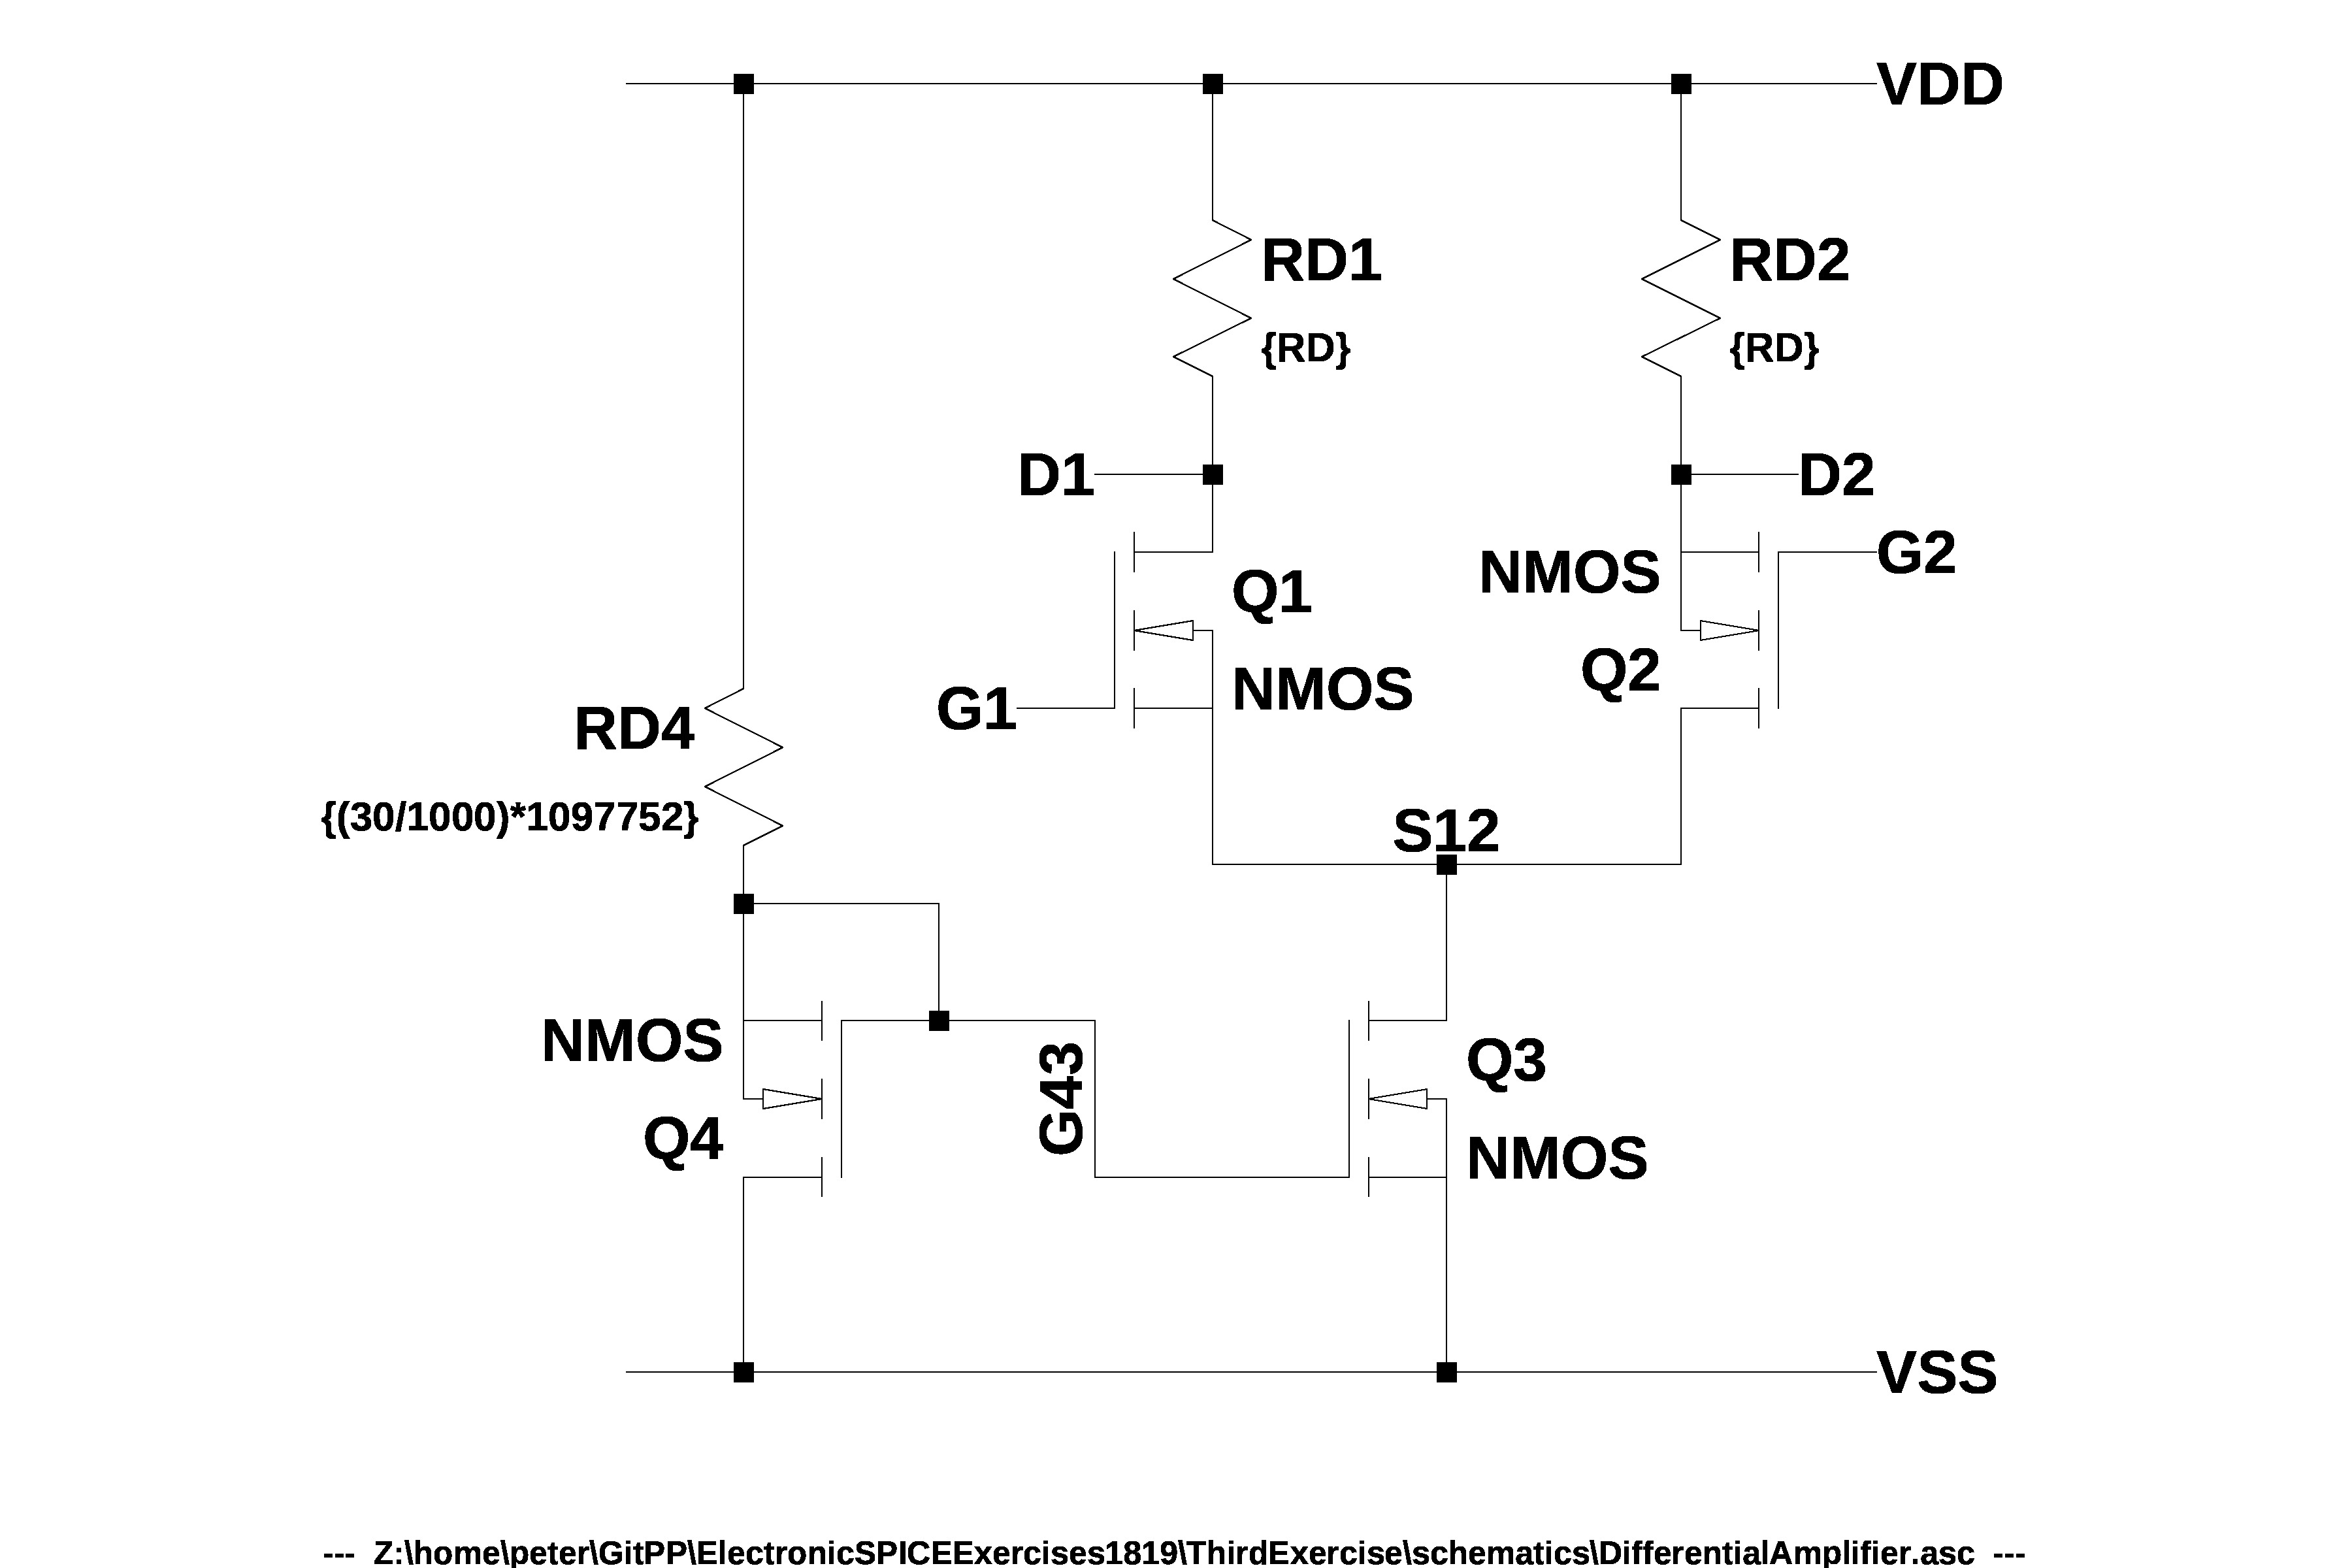
\includegraphics[width=12cm]{schematics/DifferentialAmplifier.jpg}
  \caption{Differential amplifier with MOS current source}
  \label{DifferentialAmplifier}
\end{figure}

Data:\\
\begin{align}
V_t = 0.5V\\
{K'}_n = {\mu}_n C_{ox} = 200 \frac{\mu A}{V^2}\\
\lambda = 0\\
\left(\frac{W}{L}\right)_1 = \left(\frac{W}{L}\right)_2 = 20\\
\left(\frac{W}{L}\right)_3 = \left(\frac{W}{L}\right)_4 = 5\\
R_{D_1} = R_{D_2} = 20k\Omega\\
R_{D_4} = \frac{30}{1000}\cdot 1097752 \Omega = 32.93k\Omega \simeq 33k\Omega\\
V_{DD} = 3V\\
V_{SS} = -3V
\end{align}

\section{MOSFET current mirror source - Analytic solution}
\subsection{$I_{D_4}$}
The transistor $M_4$ has a short circuit between its drain and its gate, so the transistor works in saturation mode.
The current $I_{D_4}$ could be calculated as:\\
\begin{align}
I_{D_4} &= \frac{1}{2}{K'}_n \left(\frac{W}{L}\right)_4 (V_{D_4SS} - V_t)^2 \label{ID4Sat}
\end{align}
Other expression of the current $I_{D_4}$ could be calculated using the LKT:\\
\begin{align}
V_{DD}-R_{D_4}I_{D_4}-V_{D4SS}-V_{SS} = 0 \implies
I_{D_4} = \frac{V_{DD} - V_{D_4SS} - V_{SS}}{R_{D_4}}\label{ID4K}
\end{align}
Using the equations \ref{ID4Sat} and \ref{ID4K} it's possible calculating $V_{D_4SS}$:\\
\begin{align}
\frac{1}{2}{K'}_n \left(\frac{W}{L}\right)_4 (V_{D_4SS} - V_t)^2 = \frac{V_{DD} - V_{D_4SS} - V_{SS}}{R_{D_4}}
\end{align}
\begin{align}
\frac{1}{2}\cdot 200 \frac{\mu A}{V^2} \cdot 5 \frac{\mu m}{\mu m} (V_{D_4SS} - 0.5V)^2 = \frac{3V - V_{D_4SS} - (-3V)}{33k\Omega}\\
500 \frac{\mu A}{V^2} (V_{D_4SS} -0.5V)^2 = \frac{6}{33}mA-\frac{1}{33k\Omega}V_{D_4SS}\\
500 \frac{\mu A}{V^2} (V_{D_4SS}^2- V_{D_4SS}\cdot V +0.25V^2) = \frac{6}{33}mA-\frac{1}{33k\Omega}V_{D_4SS}\\
500 \frac{\mu A}{V^2} \cdot V_{D_4SS}^2 + \left(-500 \frac{\mu A}{V^2}V + \frac{1}{33k\Omega}\right) V_{D_4SS} + 500 \frac{\mu A}{V^2} \cdot 0.25V^2 -\frac{6}{33}mA = 0\\
0.5 \frac{mA}{V^2} \cdot V_{D_4SS}^2 + \left(-0.5 \frac{mA}{V^2}V + \frac{1}{33k\Omega}\right) V_{D_4SS} + 0.5 \frac{mA}{V^2} \cdot 0.25V^2 -\frac{6}{33}mA = 0\\
\left(0.5 \frac{mA}{V^2}\right) V_{D_4SS}^2 + \left( -\frac{31}{66}\frac{mA}{V}\right) V_{D_4SS} + \left(-0.05682mA\right) = 0
\end{align}
\begin{align}
V_{{D_{4}SS}_{1,2}} = \frac{-\left( -\frac{31}{66}\frac{mA}{V}\right)\pm \sqrt{\left(-\frac{31}{66}\frac{mA}{V}\right)^2-4\cdot\left(0.5 \frac{mA}{V^2}\right)\cdot\left(-0.05682mA\right)}}{2\cdot0.5 \frac{mA}{V^2}} = 
\left\{
\begin{array}{l}
1.04784V\\
-0.10845V\\
\end{array}
\right.
\end{align}

\section{SPICE Operating Point analysis}
\lstinputlisting{netlist/DifferentialAmplifier.cir}
\lstinputlisting{netlist/DifferentialAmplifier.op}

\end{document}
